\documentclass[12pt,a4paper]{article}

\usepackage{a4wide}
\usepackage{minted}
\usepackage{csvsimple}
\usepackage{amsmath}
\usepackage{booktabs}
\usepackage{amssymb}
\usepackage{nicefrac}
\usepackage{enumitem}
\usepackage{float}
\usepackage{todonotes}
\usepackage[breaklinks,plainpages=false,pdfpagelabels]{hyperref}
\hypersetup{colorlinks,citecolor=blue,filecolor=blue,linkcolor=blue,urlcolor=blue}
\usepackage{graphicx}
\setlength\parindent{0pt} % no paragraph indents
\setlength\parskip{6pt} % paragraph vertical spacing
\usepackage{circuitikz} % for circuit diagrams
\usepackage{pgfplots}
\usepackage{tikz}
\usetikzlibrary{positioning,shapes,shadows,arrows,calc}
\DeclareMathOperator{\sinc}{sinc} %sinc
\usepackage[normalem]{ulem} %strike out text using \sout

\usepackage{fancyhdr}
\pagestyle{fancy}
\fancyhead[L]{CSSE4010: Digital Doo-Hickeys}
\fancyhead[R]{Sem 2, 2023}


%---------------------------------------------------------------%
%                                                               %
%               environment definitions                         %
%                                                               %
%---------------------------------------------------------------%
\newcounter{boldalphcounter}
\renewcommand{\theboldalphcounter}{(\alph{boldalphcounter})}
\newenvironment{boldalphlist}{\begin{list}{\textbf{\theboldalphcounter}}%
  {\usecounter{boldalphcounter}}}{\end{list}}

\newcounter{alphcounter}
\renewcommand{\thealphcounter}{(\alph{alphcounter})}
\newenvironment{alphlist}{\begin{list}{\thealphcounter}%
  {\usecounter{alphcounter}}}{\end{list}}

\newcounter{romancounter}
\renewcommand{\theromancounter}{\roman{romancounter})}
\newenvironment{romanlist}{\begin{list}{\textbf{\theromancounter}}%
  {\usecounter{romancounter}}}{\end{list}}

\newcounter{boldarabiccounter}
\renewcommand{\theboldarabiccounter}{\arabic{boldarabiccounter}}
\newenvironment{boldarabiclist}{\begin{list}{\textbf{\theboldarabiccounter.}}%
  {\usecounter{boldarabiccounter}}}{\end{list}}

 % Counter
\newcounter{questioncounter}

\begin{document}

\begin{center}
\bigskip
\section*{CSSE4010 A4}
\end{center}

David Gaul

s4671313

Lab Session: Wednesday 10-12

Submission Date: 16th-ish October

\section{Introduction}

The purpose of this practical was to  develop a finite impulse response (FIR) filter using Xilinx's Model Composer and test it's functionality. The filter was a low pass filter of the form

\[y(n) = \sum_{i=0}^{17} a_ix(n-i)\]

This filter was first developed using a filter developed through Matlab's built-in functions. Following this, two pipelines were developed for hardware equivalents: one with and the other without optimisation strategies. From here, the performance metrics of both filters were compared against each other and the software implementation.

I'm going to acknowledge that the lab reports have reduced in quality as the semester has progressed. My apologies. The quality of said reports is directly proportional to my will to live. But today we're going to have fun.

\section{Word Length Selection}

Before any hardware implementations could be commenced, it was necessary to determine the words lengths being used for fixed point decimal values. Fixed point decimal values are preferred over floating point representations because they save on space, while also improving time complexity. A properly selected fixed point word length can boost the running speed, reduce resource consumption and result in a minimal loss of accuracy. For the purposes of prac 5, two word lengths had to  be decided: the word length for the input signal and filter co-efficients.

Deciding the word length for the input signal required close analysis of the input itself. As was observed, the input was the combination of two sinusoidal signals with the functions:

\[y_1 = \sin(400\pi t)\]
\[y_2 = 4\sin(4000\pi t)\]

The minimum and maximum values of the signal were found using Matlab's min() and max() functions. These were found to be -4 and 4 respectively. In order to fully express these inputs, 4 bits is required: three bits to express '4,' and a final bit for the 2's complement.

Similarly, the minimum and maximum values of the filter co-efficients were analysed. These were found to be -0.002 and 0.1634. Only a single bit is required to before the floating point to express these: the bit for 2's complement signing. Ultimately, it was decided that the input signal would require 4 bits on the integer value of its word length, whereas the co-efficients required only 1 bit. The total word lengths of each was tested within hardware filter 1 implementation, and will be discussed within that section.

\section{Hardware Filter 1}

Although both hardware implementations show many similarities, it is worth beginning with the initial software filter to explain each architecture. In implementing the software filter via Matlab, it returned a 17th degree filter, where the filter co-efficients can be found in figure \ref{fig:coefficients}.

\begin{figure}[H]
    \centering
    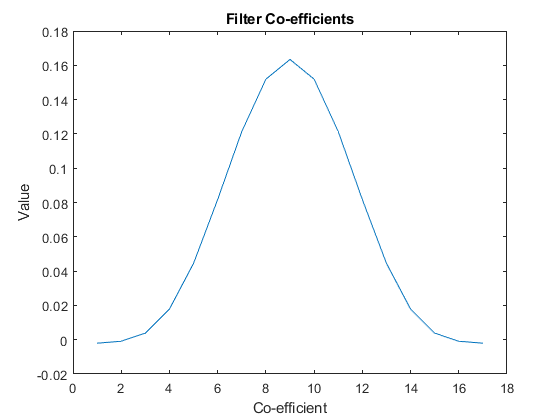
\includegraphics[scale=0.25]{images/coefficients.png}
    \caption{Polynomial co-efficient values for FIR Filter}
    \label{fig:coefficients}
\end{figure}

Transferring this simple model over to Model Composer was more or less a drag and drop process. The entire block diagram for the un-optimised filter can be found in figure \ref{fig:untuned_block}.

\begin{figure}[H]
    \centering
    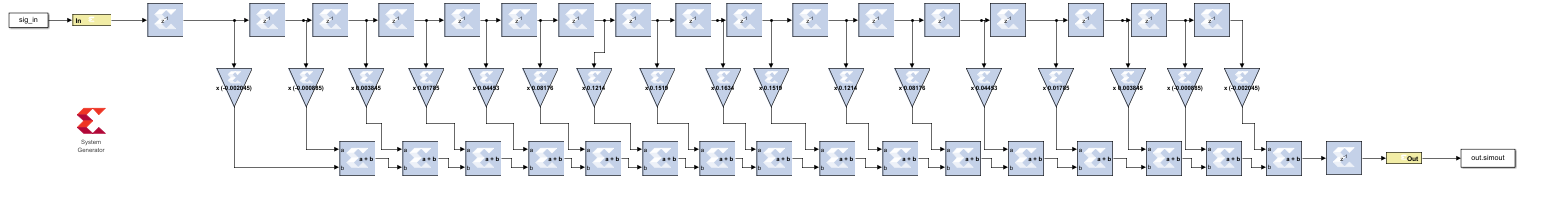
\includegraphics[scale=0.25]{images/untuned_block.PNG}
    \caption{Block diagram of the untuned filter}
    \label{fig:untuned_block}
\end{figure}

Here, it's worth mentioning that the design architecture perfectly mimics that of the provided equation at the introduction of the report. Each delay block represents a delay of $Z^{-1}$ in the Z-domain, which correlates to $x(n-1)$ in the time domain. The stacking of these delays, in combination with the summation of filter co-efficients, results in a hardware equivalent to the software implementation within the provided Matlab script. Figure \ref{fig:untuned_block_close} shows a zoomed-in view of the left-most co-efficients, which correspond with the first and second filter polynomials.

\begin{figure}[H]
    \centering
    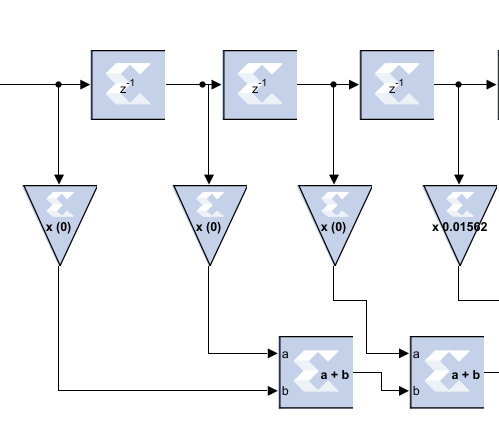
\includegraphics[scale=0.33]{images/untuned_block_close.PNG}
    \caption{Zoomed in view of the first two co-efficients for the untuned filter}
    \label{fig:untuned_block_close}
\end{figure}

With the design successfully set up, the full word lengths for the input and filter co-efficients could be determined. To determine the accuracy of hardware filter implementations, a signal to error ratio (SER) function was used. The most common SER function is:

\[SER = 10\times \log_{10}(\frac{(HW-SW)^2}{SW^2})\]

Where HW represents the hardware signal, and SW represents the software signal. 

In analysing the array of filter co-efficients, it was found that the smallest value was $8.914e^-4$. Such a number would require 14 bits to fully represent, which would indicate that a 16 bit word length would provide the most accurate results possible. However, it was acknowledged that smaller word lengths could be used with minimal loss in accuracy. To fully test the effect of word length on filter accuracy, tests were conducted over the number of bits representing the decimal value. Bit values from 3 through to 15 were used, and the results can be found in figure \ref{fig:bits_selecting}

\begin{figure}[H]
    \centering
    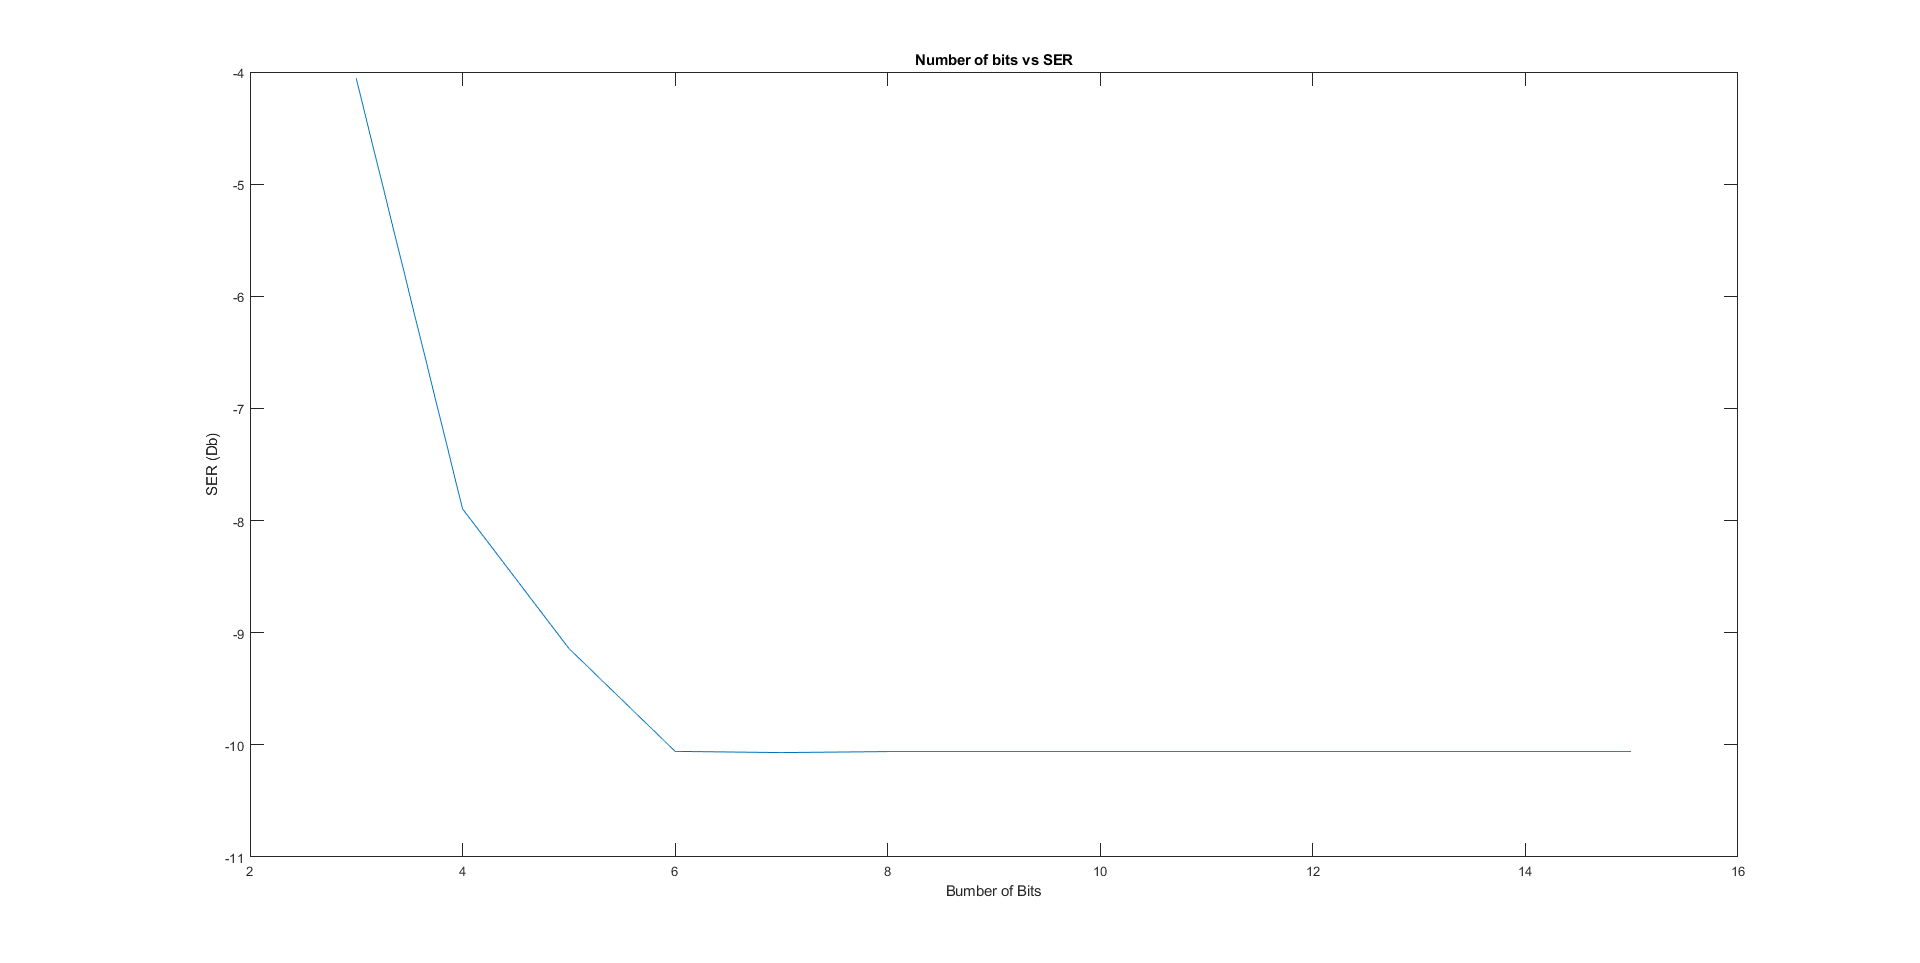
\includegraphics[scale=0.25]{images/bits_selecting.png}
    \caption{Line plot showing the reduction in SER as the number of decimal bits on the CMUL blocks increases}
    \label{fig:bits_selecting}
\end{figure}

\begin{figure}[H]
    \centering
    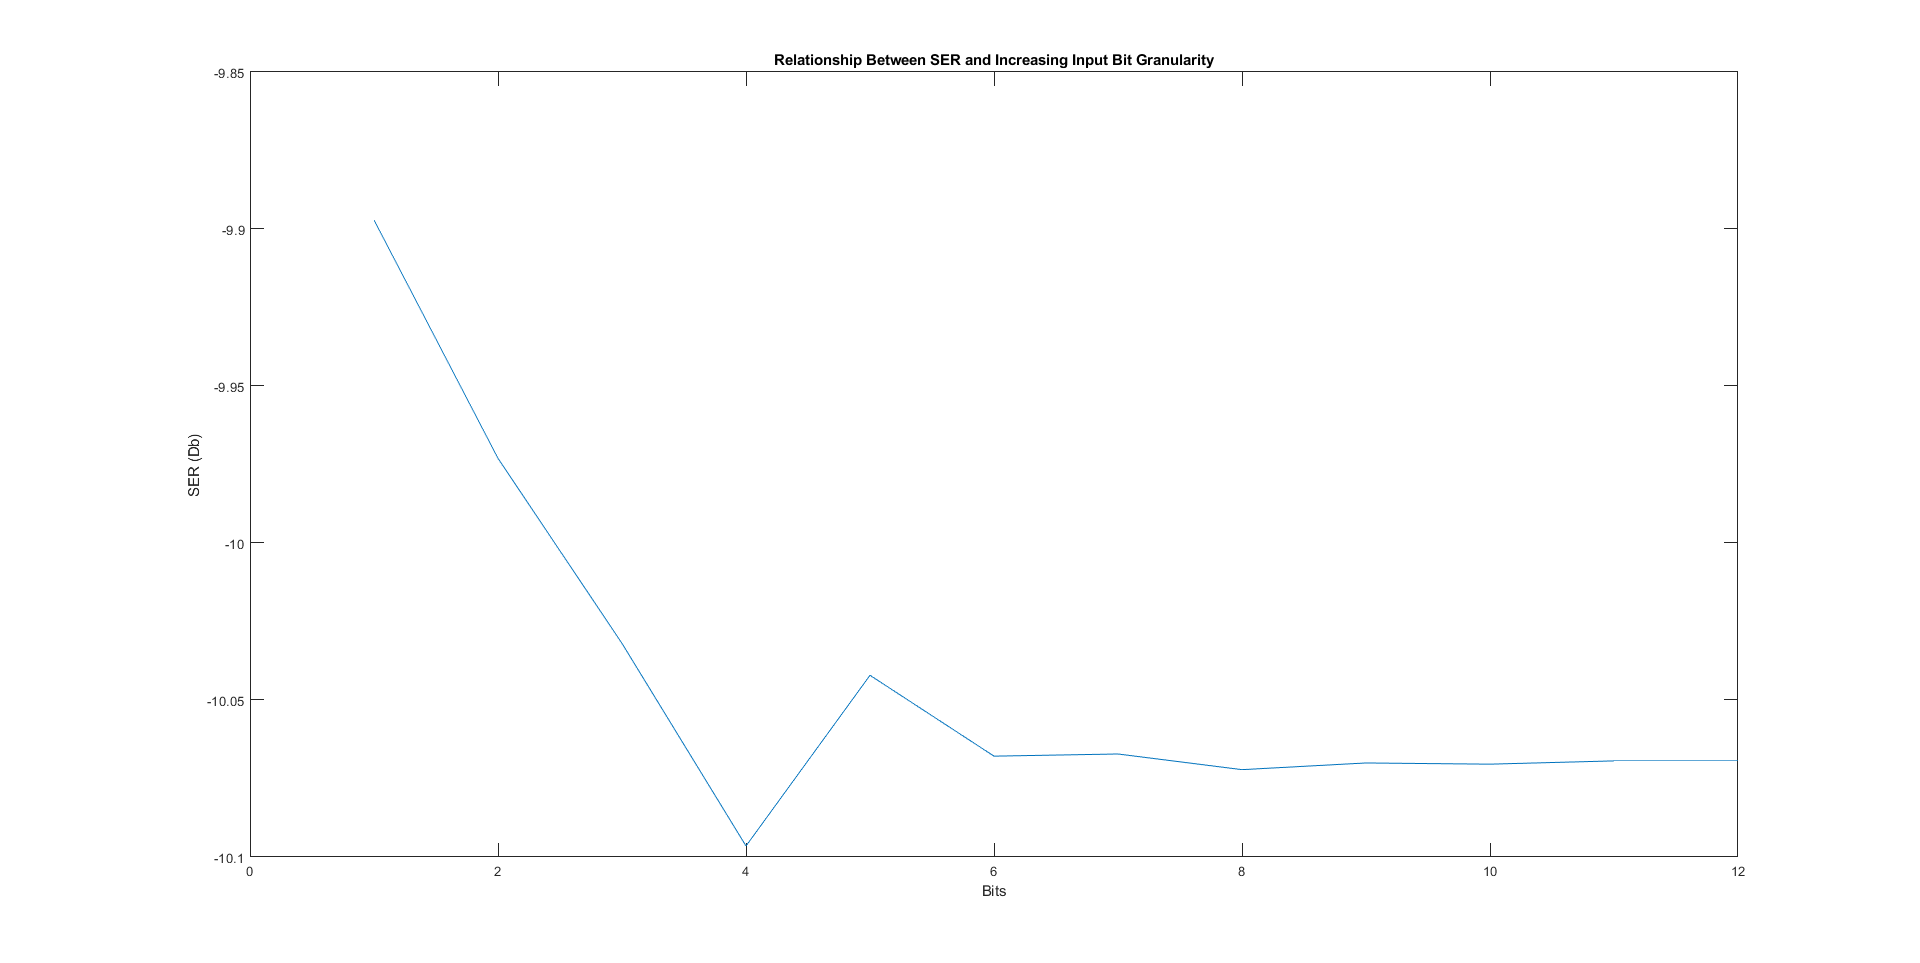
\includegraphics[scale=0.25]{images/bits_input.png}
    \caption{Line plot showing the reduction in SER as the number of decimal places on the input signal in increases}
    \label{fig:bits_input}
\end{figure}

As can be seen, minimal accuracy is gained by adding more values past 6 decimal places. Conversely, it does add more complexity and runtime. For this reason, the word-length of the filter co-efficients was determined to be 7: 1 bit for the signed value, and 6 bits for the decimal value. Through similar testing, it was found that the optimum word length for the input signal was 8 bits: 4 for the integer value and 4 for the decimal value. The derivation of SER values for the input word length can be found in figure \ref{fig:bits_input}

The optimisation of these final values can be verified by comparing the obtained hardware signal to the original software filter. Figure \ref{fig:sw_untuned} shows that the solutions are nearly identical. 

\begin{figure}[H]
    \centering
    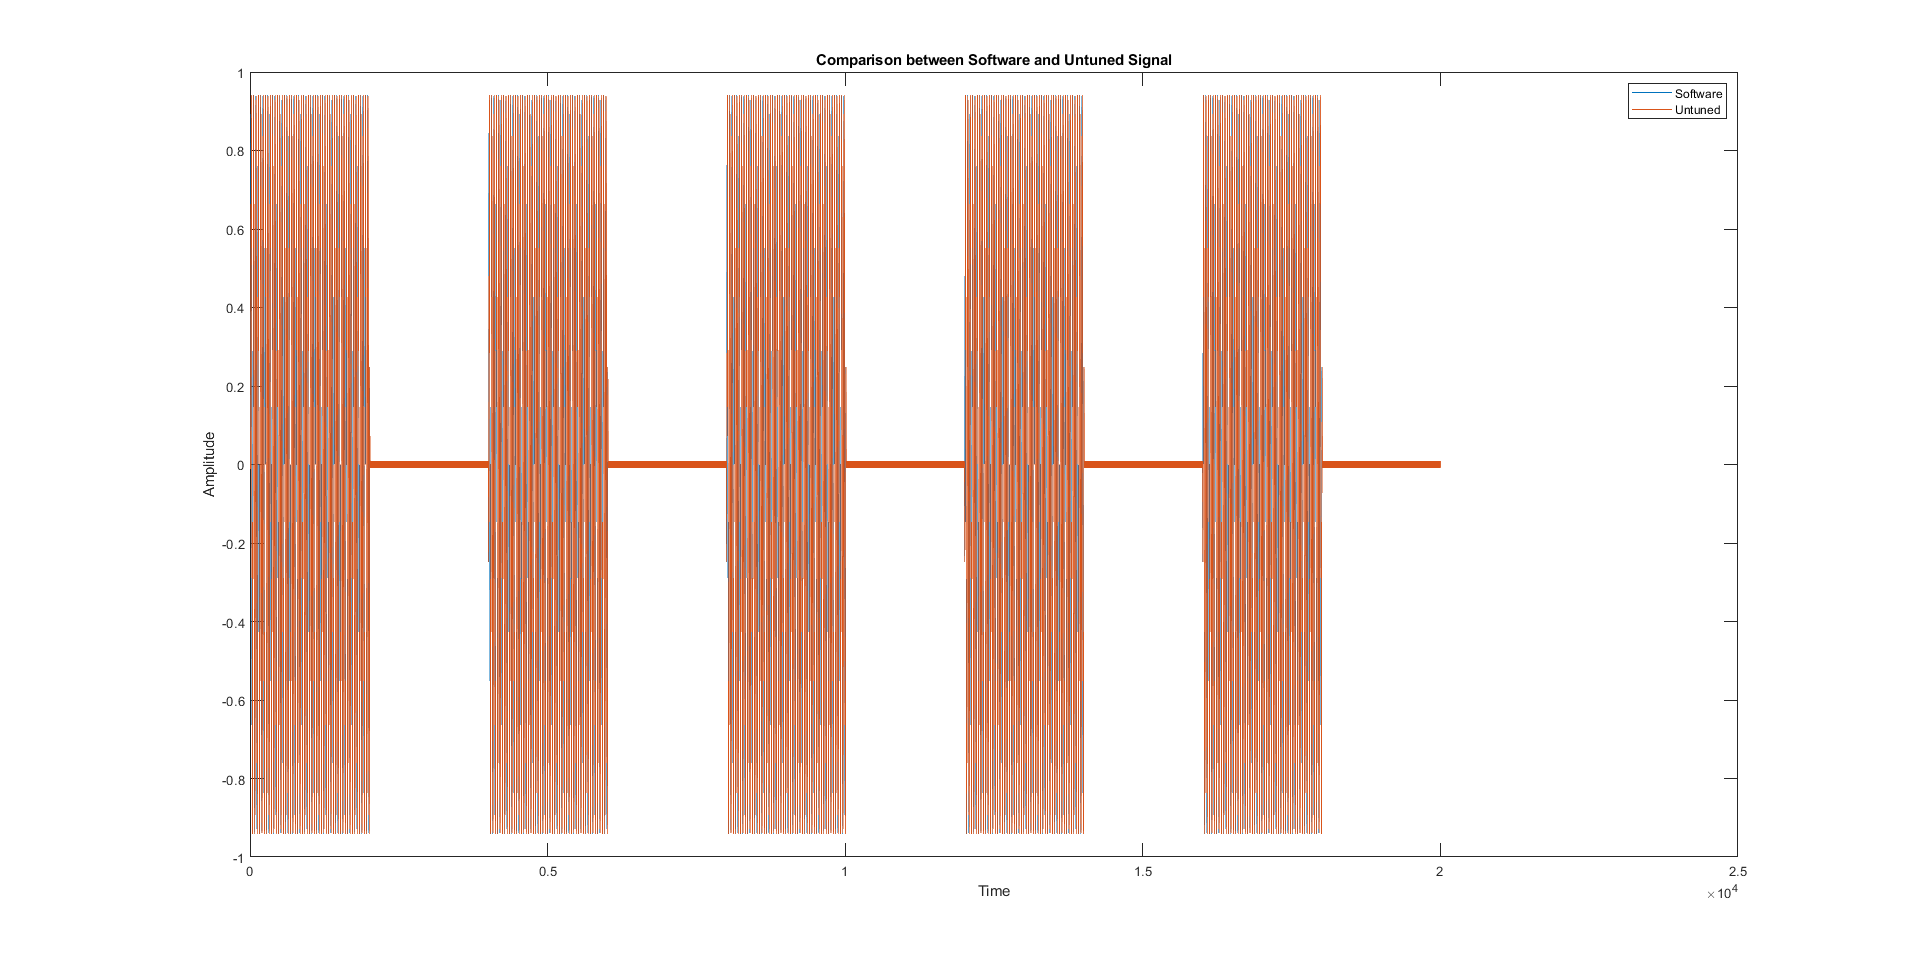
\includegraphics[scale=0.25]{images/sw_untuned.png}
    \caption{Comparison of software and untuned hardware filters}
    \label{fig:sw_untuned}
\end{figure}

Close inpection of these signal reveals that there is a delay on the hardware signal. This is due to the implementation of delay blocks within the Simulink model. As these are mandatory to retain system synchronicity, this delay is unavoidable. Figure \ref{fig:sw_untuned_close} shows a zoomed-in view of this delay. 

\begin{figure}[H]
    \centering
    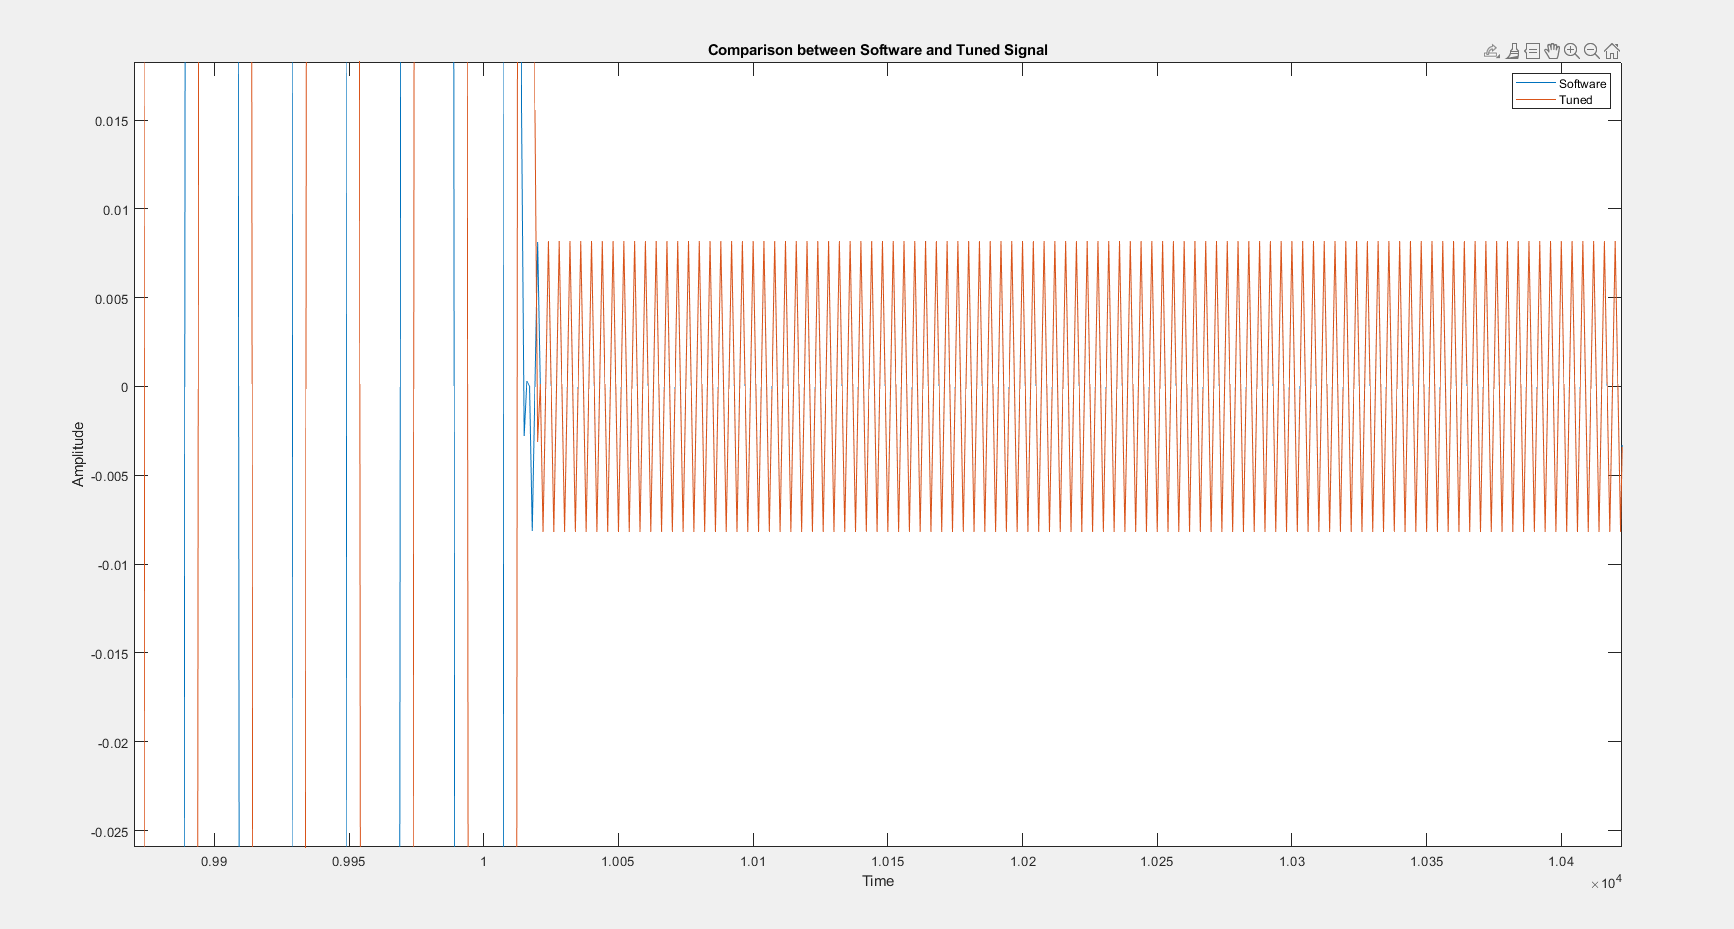
\includegraphics[scale=0.25]{images/sw_tuned_close.PNG}
    \caption{Zoomed in view of software and untuned filter comparison. This highlights the slight delay present for the hardware filter}
    \label{fig:sw_untuned_close}
\end{figure}

With successful verification of the hardware implementation's functionality, its runtime metrics could be recorded. Figure \ref{fig:timing_results_untuned} shows the timing schedule for model synthesis. As could be seen, all pathways were able to run in under 5ns and model synthesis was successful. The critical path can be observed in figure \ref{fig:critical_untuned}

\begin{figure}[H]
    \centering
    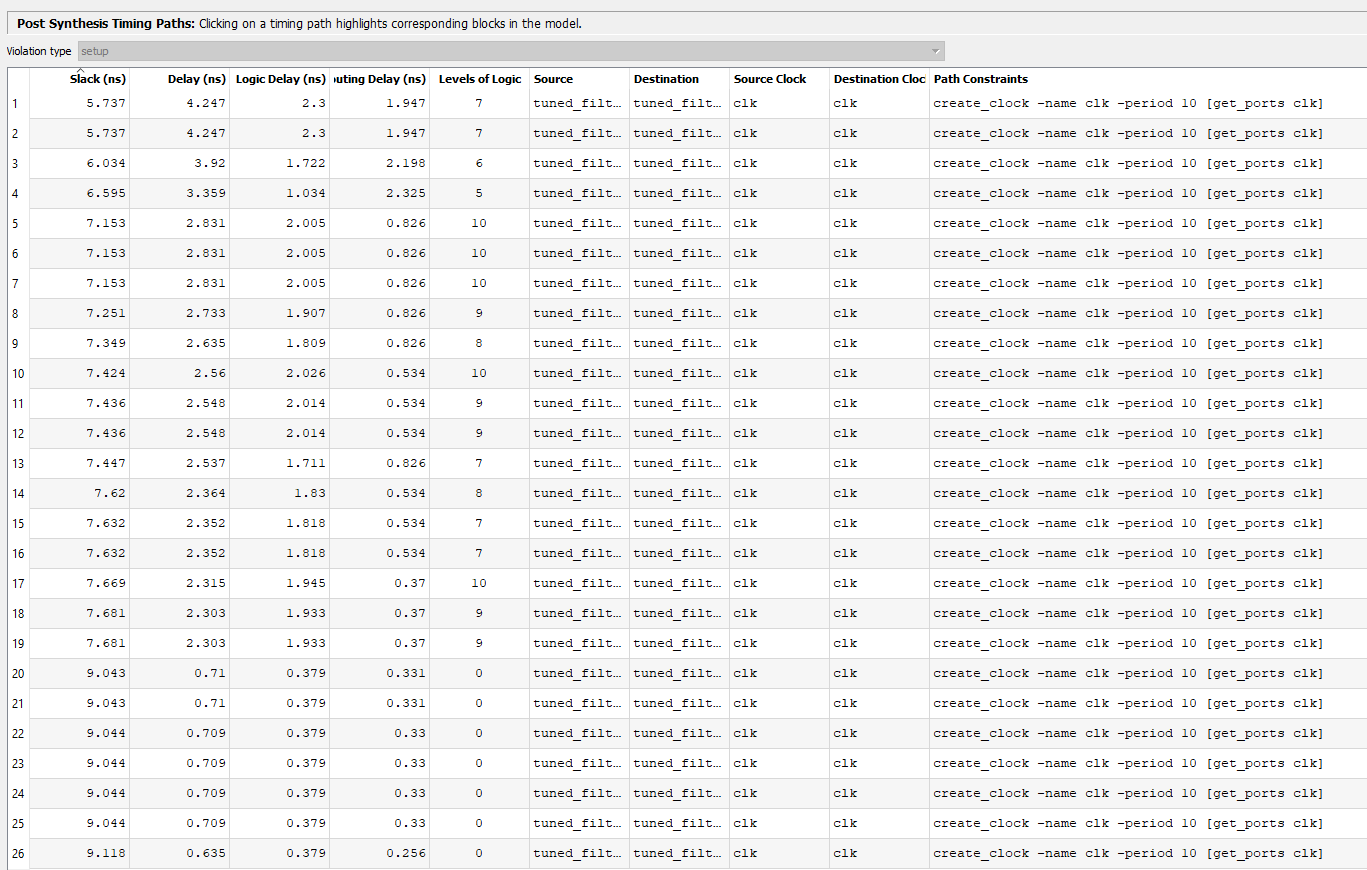
\includegraphics[scale=0.25]{images/timing_results_untuned.PNG}
    \caption{Timing results of the untuned filter. Note that all paths have run in passing time}
    \label{fig:timing_results_untuned}
\end{figure}

\begin{figure}[H]
    \centering
    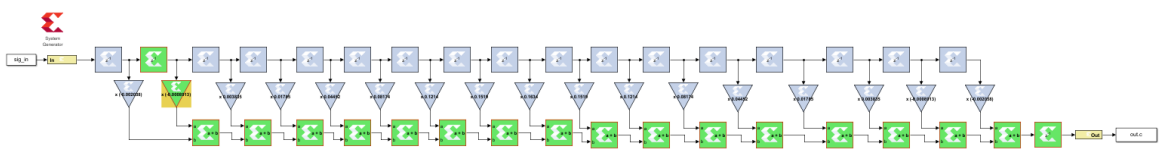
\includegraphics[scale=0.25]{images/untuned_critical.PNG}
    \caption{Critical path for the untuned model}
    \label{fig:critical_untuned}
\end{figure}

The memory utilisation of the model was found by copying and synthesizing the generated .vhdl code created by model composer. The utilisation report can be found in figure \ref{fig:untuned_utilisation}

\begin{figure}[H]
    \centering
    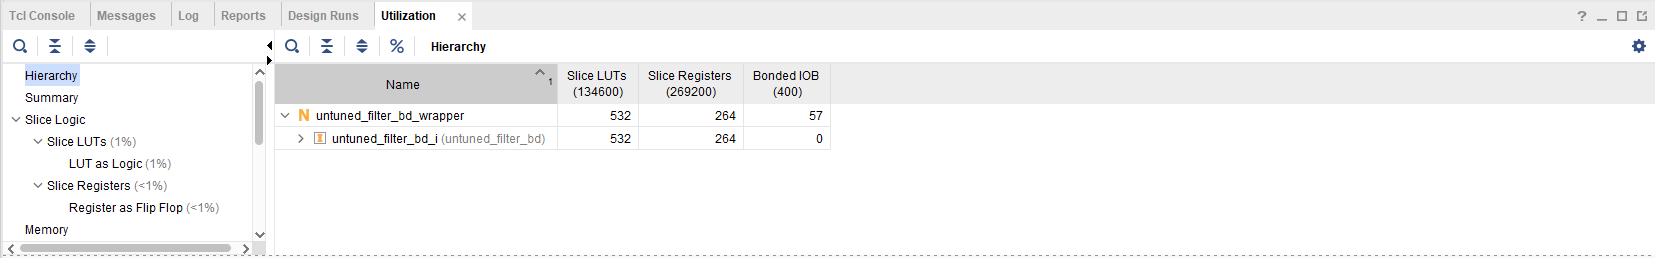
\includegraphics[scale=0.33]{images/untuned_utilisation.PNG}
    \caption{Memory utilisation of the untuned filter}
    \label{fig:untuned_utilisation}
\end{figure}

At the end of the first hardware filter, it was found that it could almost perfectly replicate the software filter with a critical path delay of 4.3ns and a memory utilisation of 532 LUTs: less than 1$\%$ of the available resources.

\section{Hardware Filter 2}

Although it was established that the first pipeline worked, there were several optimisation issues. Due to the lack of optimisation, the filter ran slower and consumed more resources than was necessary. Careful analysis showed that there were two main ways of optimising this initial filter:

\begin{itemize}
    \item Pipelining - Used to parallelise computations and reduce reliance on delays.
    \item Data broadcasting - Using the same filter co-efficients in multiple areas.
\end{itemize}

Data broadcasting was possible due to the nature of the filter co-efficients. Figure \ref{fig:coefficients} shows that a mirror image of co-efficient values is created by the software filter. Computed values could therefore be recycled and implemented later in the FIR filter. Finally, delay blocks could also be removed by integrating them into the CMUL and AddSub blocks. The fully optimised hardware filter can be found in figure \ref{fig:tuned_block}.

\begin{figure}[H]
    \centering
    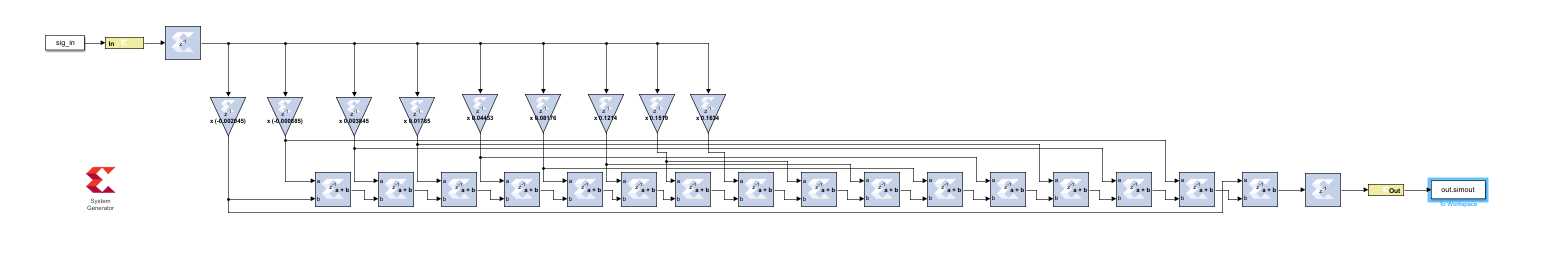
\includegraphics[scale=0.25]{images/tuned_block.PNG}
    \caption{Block diagram of tuned filter}
    \label{fig:tuned_block}
\end{figure}

Figure \ref{fig:tuned_block_close} shows a close-up view of the first two co-efficients for this block diagram.

\begin{figure}[H]
    \centering
    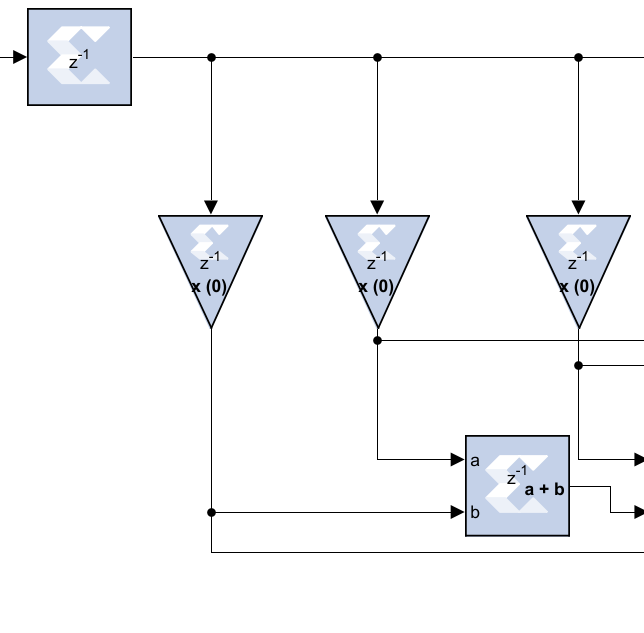
\includegraphics[scale=0.33]{images/tuned_block_close.PNG}
    \caption{Close up view of the first two filter co-efficients for the tuned filter}
    \label{fig:tuned_block_close}
\end{figure}

Since the values for the input signal and co-efficients remained unchanged between filter iterations, updating word lengths was unnecessary. 

Which can be further verified by figure \ref{fig:sw_tuned} which compares the tuned filter to the original software implementation.

\begin{figure}[H]
    \centering
    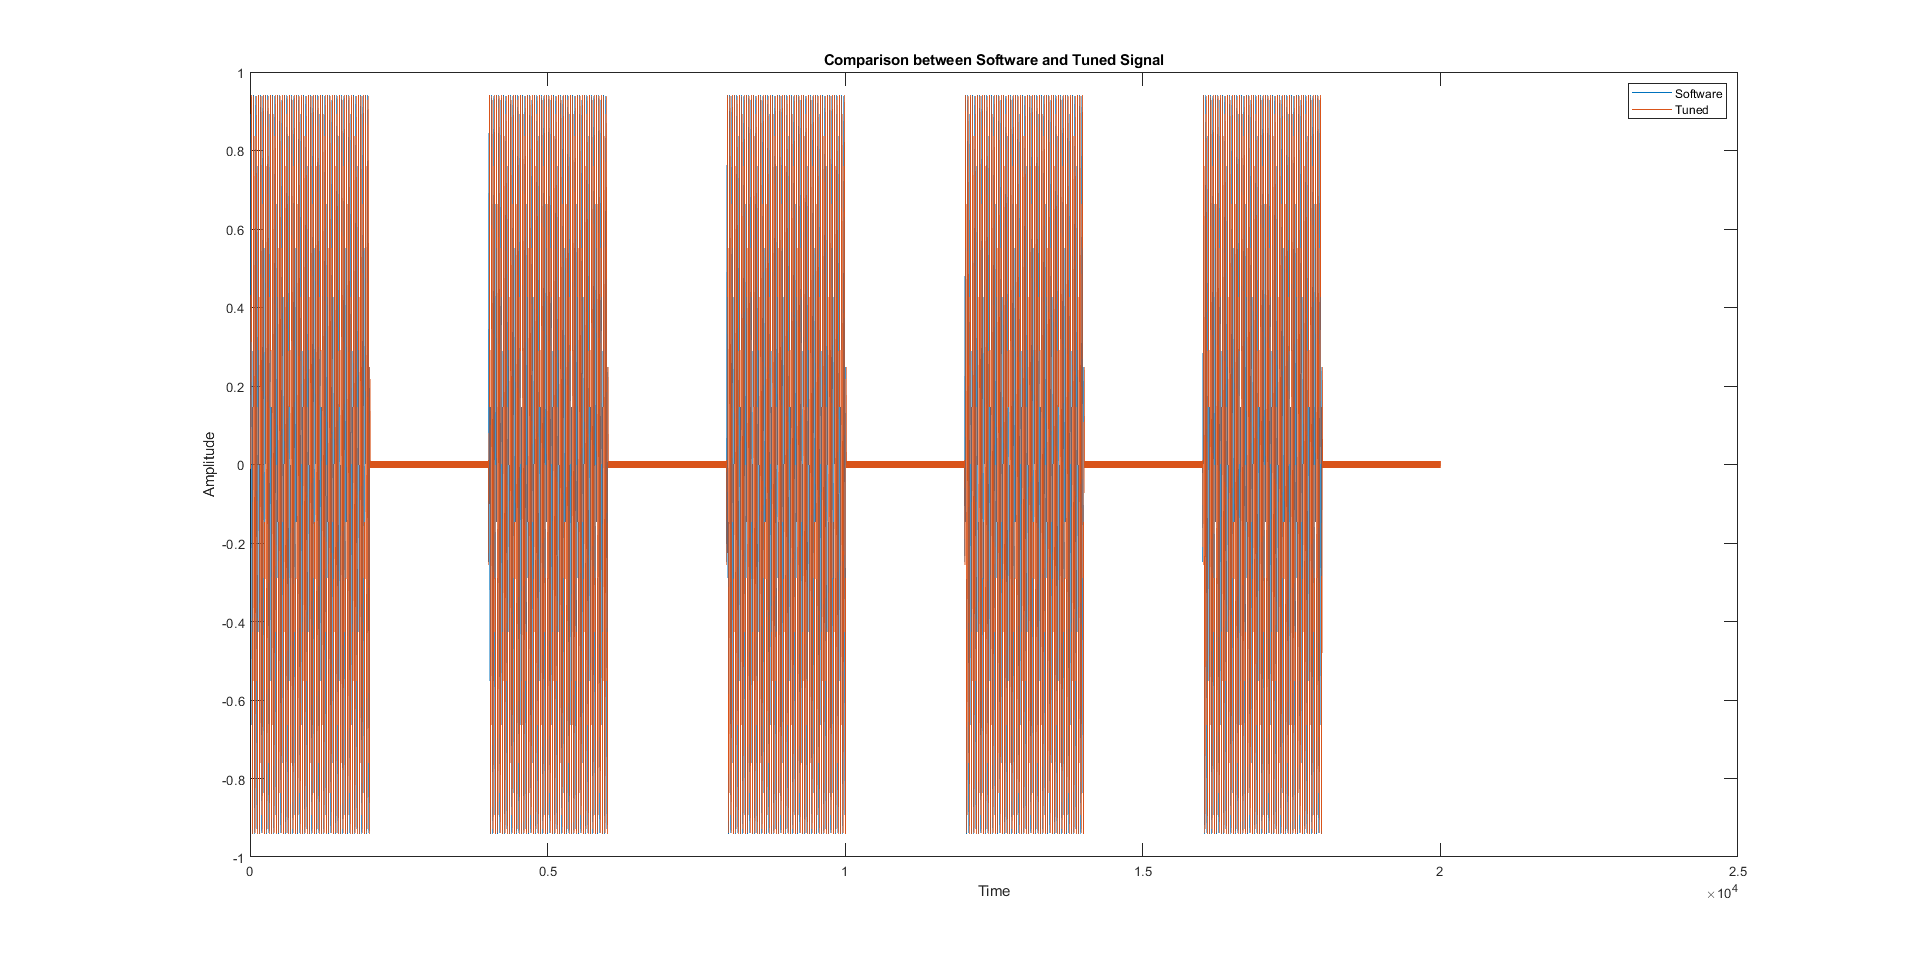
\includegraphics[scale=0.25]{images/sw_tuned.png}
    \caption{Output comparison between the software and tuned hardware filters.}
    \label{fig:sw_tuned}
\end{figure}

However, a zoomed in view of the output indicates that there is more delay in the output. This is due to the integration of latency within the CMUL and AddSub blocks. Because of this, the critical path delay had been changed. Figure \ref{fig:sw_tuned_close} shows the timing report of Model Composer synthesizing.

\begin{figure}[H]
    \centering
    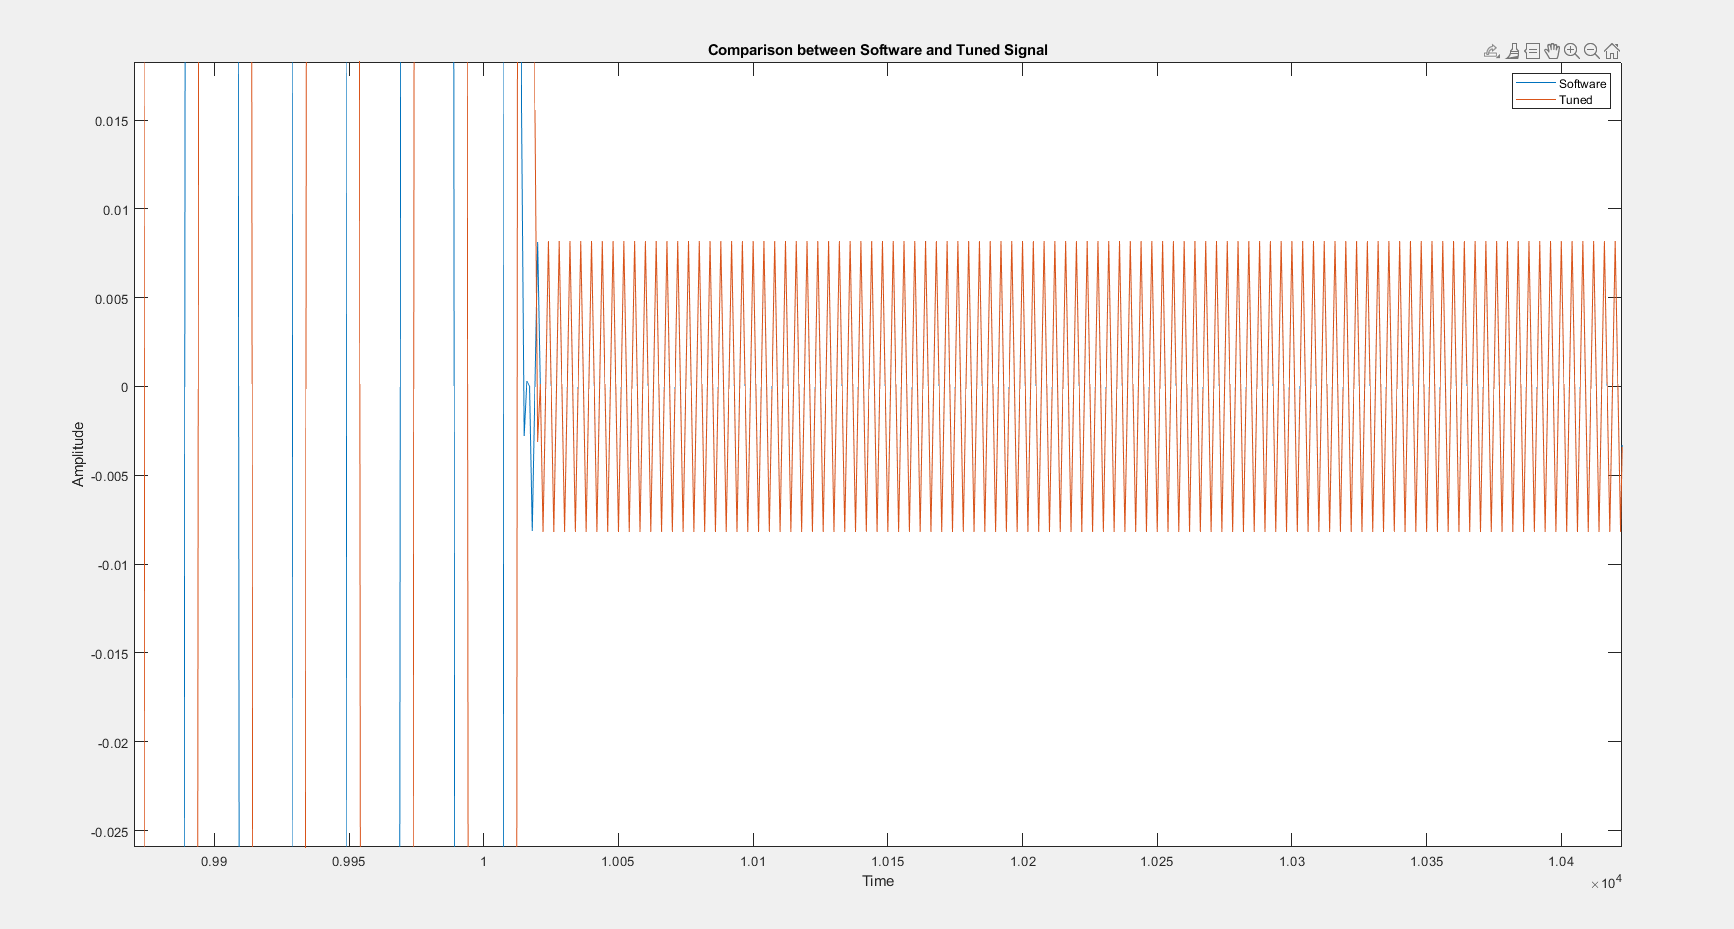
\includegraphics[scale=0.25]{images/sw_tuned_close.PNG}
    \caption{Zoomed in view of the software and tuned hardware filters highlighting the delay between them}
    \label{fig:sw_tuned_close}
\end{figure}

Although the critical path remained unchanged for the tuned filter, the average running speed for each path was increased. The critical path delay for the tuned pipeline could be found within figure \ref{fig:timing_results_tuned}.

\begin{figure}[H]
    \centering
    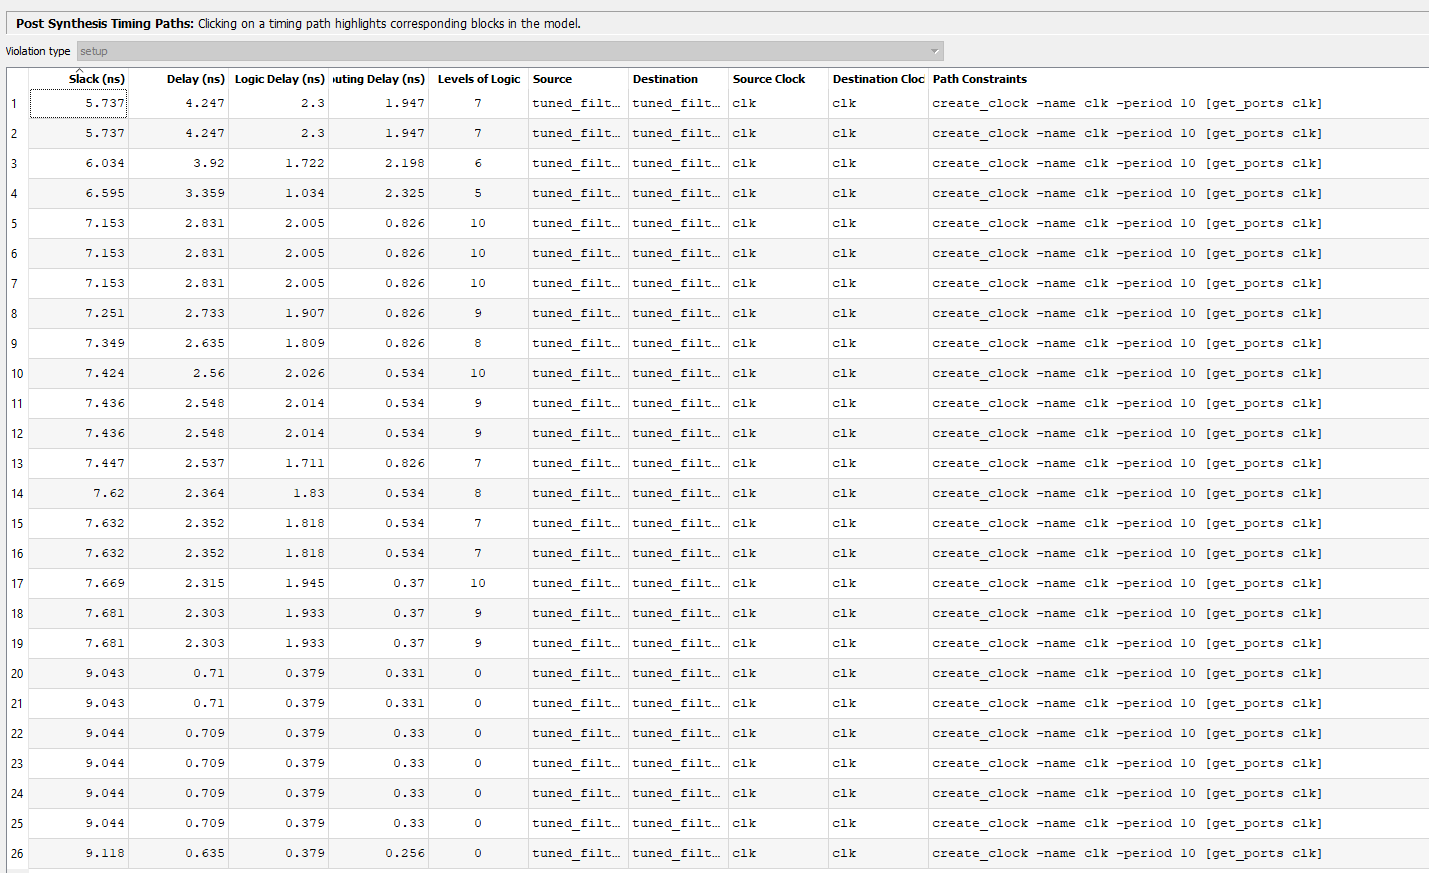
\includegraphics[scale=0.25]{images/timing_results_tuned.PNG}
    \caption{Total timing results for the tuned filter. All paths are able to evaluate within passing time.}
    \label{fig:timing_results_tuned}
\end{figure}

\begin{figure}[H]
    \centering
    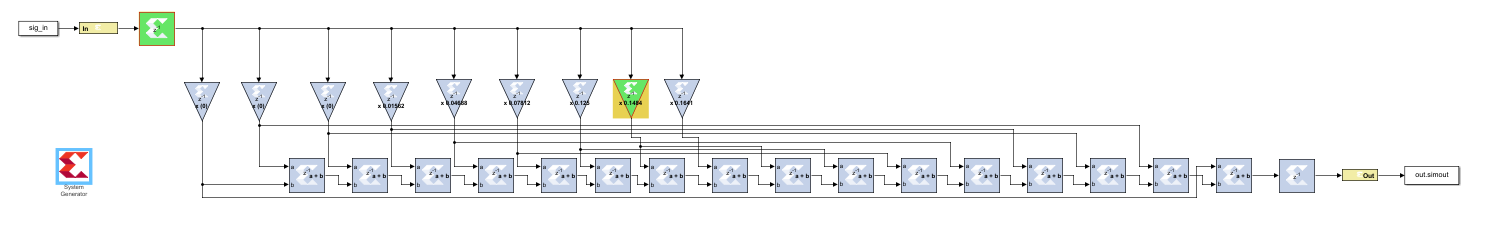
\includegraphics[scale=0.25]{images/critical_path_tuned.PNG}
    \caption{Critical path delay of the tuned system}
    \label{fig:critical_path_tuned}
\end{figure}

Lastly, the memory utilisation for the tuned model can be found within figure \ref{fig:tuned_utilisation}

\begin{figure}[H]
    \centering
    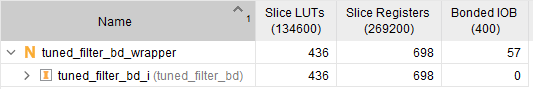
\includegraphics[scale=0.25]{images/tuned_utilisation.PNG}
    \caption{Memory consumption of tuned filter}
    \label{fig:tuned_utilisation}
\end{figure}

\section{Model Comparison}

After comparing both models, several notable observations surfaced. The first of these is that both the tuned and untuned filters were able to filter equally as accurately on the input signal. However, the tuned filter was able to outperform the untuned implementation in terms of runtime and area complexity. In implementing pipelining and broadcasting, the memory utilisation was able to be reduced from 532 to 436 LUTs; a 20$\%$ reduction in memory utilisation. Furthermore, although the critical path delay remained unchanged between implementations, the tuned model generally had on average less delay and more slack for each of its paths.

In total, optimising the model reduced memory utilisation while increasing running speed.

\section{Conclusion}

In conclusion, the system worked as expected. It was found that, quite unsurprisingly, a tuned filter can outperform un-optimised variants in terms of runtime and memory utilisation, with no loss in accuracy. Furthermore, hardware implementations can have the word lengths of their inputs adjusted to further increase this speed and memory optimisation. This, however, comes at the cost of reducing accuracy. Careful tuning is necessary to find the perfect balance between these parameters. 

Anyway, job done. Product worked. This is the final prac report required for my time in CSSE4010. Thanks for marking. God bless.

xoxo

\end{document}
